To improve the purity of selected electrons further additional identification are applied suppress backgrounds such electrons from hadronic jets, converted photons, non-prompt electrons from heavy-flavor decays. This is done via a likelihood based discriminant built from ID and calorimeter measurements. The identification is done using a likelihood-based discriminant using PDFs created from 13 smoothed histograms corresponding to the 13 discriminating input variables. 

Separate PDFs are created for signal and background in 9 bins of $\eta$ and 7 bins of $\et$. Signal PDFs are derived from $Z\rightarrow e^{+}e^{-}$ decays and are compared to backgrounds that mimic prompt electrons. Each reconstructed electron is assigned a likelihood value, those with higher values are classified as electrons. 

The required likelihood value to be considered an electron is rather arbitrary, so three working points (WPs) have been developed by the electron combined performance (CP)~\cite{ATLAS:EGAMPublic} group to select electrons at differing efficiencies. As the likelihood value increases, the purity of selected electrons increases with a decreasing efficiency and vice versa. 

Three of these working points are: Loose (96\% efficiency), MediumLLH (94\% efficiency), and TightLLH (88\% efficiency)\@. Figure~\ref{fig:reco_electron_id_eff} shows the electron identification efficiency in data in bins of $\et$ and $\eta$.

\begin{figure}
  \centering
  \subfloat[Electron ID efficiency as functon of $\pt$]{
    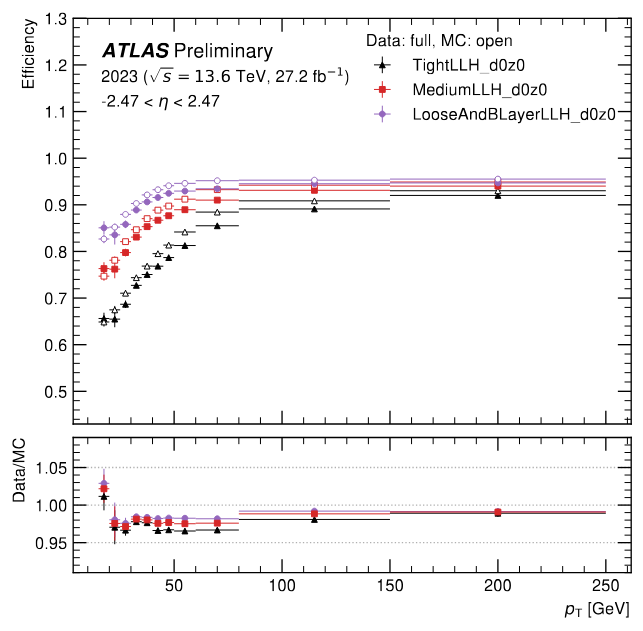
\includegraphics[width=0.45\textwidth]{figures/reco/reco_electron_id_eff_pt.png}\label{fig:reco_electron_id_eff_pt}
  }\hspace{0.01\textwidth}
  \subfloat[Electron ID efficiency as functon of $\eta$]{
    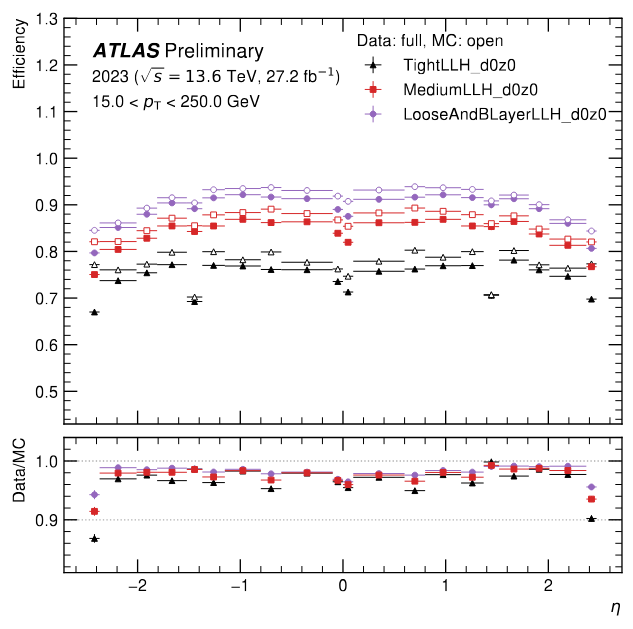
\includegraphics[width=0.45\textwidth]{figures/reco/reco_electron_id_eff_eta.png}\label{fig:reco_electron_id_eff_eta}
  }
  \caption{Electron identification efficiency in data as a function of $\pt$ (left) and $\eta$ (right) for the TightLLH, MediumLLH, and LooseAndBLayerLLH\@. The efficiency is defined as the fraction of reconstructed electrons that pass the electron identification criteria. The figure is taken from~\cite{ATLAS:EGAM-2025-04}.}\label{fig:reco_electron_id_eff}
\end{figure} 